\documentclass[11pt]{article}
\usepackage{mathpazo}
\usepackage{graphicx}
\usepackage[explicit]{titlesec}
\graphicspath {{Images/}}

	\titleformat{\section}[display]
  {\normalfont\scshape\Huge}
  {\hspace*{-70pt}\thesection.~#1}
  {-15pt}
  {\hspace*{-110pt}\rule{\dimexpr\textwidth+80pt\relax}{3pt}\Huge}

\titleformat{name=\section,numberless}[display]
  {\normalfont\scshape\Huge}
  {\hspace*{-70pt}#1}
  {-15pt}
  {\hspace*{-110pt}\rule{\dimexpr\textwidth+80pt\relax}{3pt}\Huge}
\titlespacing*{\section}{0pt}{0pt}{30pt}	


\begin{document}
		 
	 \begin{center}
 	 	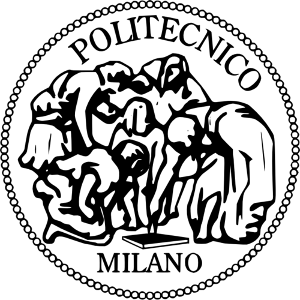
\includegraphics[scale=0.5]{Images/PolimiLogo.png}
	 \end{center}

	 \begin{center}
	 	{\Huge Politecnico di Milano}\\
	 	\vspace{5mm}
		{\Large A.A 2016-2017} 
		\vspace{5mm}\\
		{\huge Requirements Analysis and Specifications Document}   
		\vspace{5mm}\\
		{\large Version 1.0}  
     \end{center}
     
     \begin{center}
 	 	
\includegraphics[scale=1]{Images/logoPowerEnjoy.png}\\
	 \end{center}
	 	\vspace{5mm}
	
	 \begin{center}
	 	{\Large Instructor : Prof. Di Nitto}
	 	\vspace{5mm}\\	 
	 	{\Large Authors:}\\
	 	{\Large Amico Simone}\\
	 	{\Large Chianella Claudia Beatrice}\\
	 	{\Large Giovanakis Yannick}
	 \end{center}
	 
	 \newpage
	 
	 \tableofcontents{}
	 
	 \newpage
	 
	 \section{\Large Introduction}
	 
	 \subsection{Purpose}
		The aim of this document	is to give an overview of the 	requirements and specifications of system to be developed. 
		The goal of the document is to describe in detail all functional and non-functional requirements of the system, analyzing the needs of the customer and explaining common use case scenarios.
		It will set a baseline for project planning and cost estimation, giving a detailed insight to all stakeholders and future people involved in the project.
	 
	 \subsection{System}
	 The to be developed software system provides a complete support to the new PowerEnjoy car-sharing service. It will allow users to register ,log-in and use the car sharing service within the limits provided by the below specifications.
	 
	 \subsection{Aim}
	The new PowerEnjoy software system will allow visitors to register and retrieve all necessary information of common domain ( ToS , contact information...). \\Once the visitor has successfully registered to the system, he will be provided with a unique username-password combination. This enables an user to log into the system at any time , from any mobile device. \\Once logged in, the user can search within a certain distance for vehicles based on his/hers current location or based on an input address. 
	Eventually the user chooses to reserve an available vehicle, which can be picked-up within a time span of one hour.\\ 
	Should the user not pick-up the car within the one hour availability limit, then the system will tag the vehicle as available and charge the user a fee of 1 Euro.\\
	Should the user reach the car within the limit,he/she must be able to  interact with the system in order to unlock the vehicle and grant the user access to the car.
	As soon as the engine ignites,the system starts charging the user for a given amount of money per minute. The current charge will be notified through a display inside the car.\\
	The system stops charging the user as soon as the car is parked in a safe area and the user exits the car. At this point the system will automatically lock the car.
	Should the user stop in a non-safe area he/she won't be granted to end the transaction and will be charged until  he/she parks in a safe area.
	The set of safe area parking spots is defined inside the system and must be available all the time to the user's knowledge through the on-board display.
	 
	 \subsection{Actors}
	  
	\begin{itemize}
 	 	\item \textit{Visitor}: a visitor is defined as a person who is not logged into the system. A visitor can see only the log-in page with a registration form and some common information ,such as the company's customer office contact information and terms of service.
  		\item \textit{Registered User}: is defined as any person using the system who is also logged into the system. A registered user can perform any of the above mentioned actions.
  		\item \textit{Car}: is defined as the vehicle to be used by a registered user. A car must be able to communicate to with the system all the time. If a car is available (i.e currently not reserved by a registered user) then its current location must be stored in the system so to be shown on all users' devices. As soon as the engine ignition starts , the car must time the vehicle's usage in order to charge the user the right amount of money. Once the user has parked the car inside a safe area and has exited, the car informs the system about the fee to charge ,locks the doors automatically and finally informs the system that it is available again.
	\end{itemize}
	
	 \subsection{Goals}
	 \subsection{Reference Documents}
	 \subsection{Document overview}




	 	 


	 	
	
	 
     
    
     
	
\end{document}